\documentclass[14pt, a4paper]{extarticle}
\usepackage{GOST}
\usepackage{array}
\usepackage{verbatim}
\usepackage[detect-all]{siunitx}
\usepackage{amsmath}
\usepackage{amssymb}
\usepackage[utf8]{inputenc}
\usepackage{hyperref}

\usepackage{ifthen}


\usepackage{tempora}



\makeatletter
\renewcommand\@biblabel[1]{#1.}
\makeatother

% Для листинга кода:
\usepackage{listings}
\lstset{ %
	language=c++,                 % выбор языка для подсветки (здесь это С)
	basicstyle=\small\sffamily, % размер и начертание шрифта для подсветки кода
	numbers=left,               % где поставить нумерацию строк (слева\справа)
	numberstyle=\tiny,           % размер шрифта для номеров строк
	stepnumber=1,                   % размер шага между двумя номерами строк
	numbersep=5pt,                % как далеко отстоят номера строк от подсвечиваемого кода
	showspaces=false,            % показывать или нет пробелы специальными отступами
	showstringspaces=false,      % показывать или нет пробелы в строках
	showtabs=false,             % показывать или нет табуляцию в строках
	frame=single,              % рисовать рамку вокруг кода
	tabsize=2,                 % размер табуляции по умолчанию равен 2 пробелам
	captionpos=t,              % позиция заголовка вверху [t] или внизу [b] 
	breaklines=true,           % автоматически переносить строки (да\нет)
	breakatwhitespace=false, % переносить строки только если есть пробел
	escapeinside={\#*}{*)}   % если нужно добавить комментарии в коде
}


%для графиков
\usepackage{pgfplots}
\usepackage{filecontents}
\usetikzlibrary{datavisualization}
\usetikzlibrary{datavisualization.formats.functions}
\begin{filecontents}{Bubble1.dat}
	100 25
	200 90
	300 253
	400 440
	500 671
\end{filecontents}

\begin{filecontents}{Insertion1.dat}
	100 2.2
	200 2.3
	300 3.8
	400 4.2
	500 5.8
\end{filecontents}

\begin{filecontents}{Choices1.dat}
	100 24.5
	200 86
	300 230
	400 397
	500 602
\end{filecontents}


\begin{filecontents}{Bubble2.dat}
	100 55
	200 214
	300 507
	400 915
	500 1401
\end{filecontents}

\begin{filecontents}{Insertion2.dat}
	100 43
	200 192
	300 415
	400 739
	500 1144
\end{filecontents}

\begin{filecontents}{Choices2.dat}
	100 23
	200 130
	300 240
	400 450
	500 691
\end{filecontents}

\begin{filecontents}{Bubble3.dat}
	100 45
	200 193
	300 435
	400 767
	500 1095
\end{filecontents}

\begin{filecontents}{Insertion3.dat}
	100 22
	200 91
	300 189
	400 359
	500 585
\end{filecontents}

\begin{filecontents}{Choices3.dat}
	100 29
	200 113
	300 241
	400 416
	500 678
\end{filecontents}

\begin{document}
	
	\begin{table}[ht]
		\centering
		\begin{tabular}{|c|p{400pt}|} 
			\hline
			\begin{tabular}[c]{@{}c@{}} 
\includegraphics[scale=1]{baum.jpg} \\\end{tabular} &
			\footnotesize\begin{tabular}[c]{@{}c@{}}\textbf{Министерство~науки~и~высшего~образования~Российской~Федерации}\\\textbf{Федеральное~государственное~бюджетное~образовательное~учреждение}\\\textbf{~высшего~образования}\\\textbf{«Московский~государственный~технический~университет}\\\textbf{имени~Н.Э.~Баумана}\\\textbf{(национальный~исследовательский~университет)»}\\\textbf{(МГТУ~им.~Н.Э.~Баумана)}\\\end{tabular}  \\
			\hline
		\end{tabular}
	\end{table}
	\noindent\rule{\textwidth}{4pt}
	\noindent\rule[14pt]{\textwidth}{1pt}
	\hfill 
	\noindent
	\makebox{ФАКУЛЬТЕТ~}%
	\makebox[\textwidth][l]{\underline{~«Информатика и системы управления»~~~~~~~~~~~~~~~~~~~~~~~~~~~~~~~~~}}%
	\\
	\noindent
	\makebox{КАФЕДРА~}%
	\makebox[\textwidth][l]{\underline{~«Программное обеспечение ЭВМ и информационные технологии»~}}%
	\\
	
	\begin{center}
		\vspace{1.5cm}
		{\bf\huge Отчёт\par}
		{\bf\Large по лабораторной работе № 3\par}
		\vspace{0.7cm}
	\end{center}
	
	
	\noindent
	\makebox{\large{\bf Название:}~~~}
	\makebox[\textwidth][l]{\large\underline{~Алгоритмы сортировки~~~~~~~~~~~~~}}\\
	
	\noindent
	\makebox{\large{\bf Дисциплина:}~~~}
	\makebox[\textwidth][l]{\large\underline{~Анализ алгоритмов~~~~~~~~~~~~~~~~~~~~~~~~~~}}\\
	
	\vspace{1.5cm}
	\noindent
	\begin{tabular}{l c c c c c}
		Студент      & ~ИУ7-55Б~               & \hspace{2.5cm} & \hspace{2cm}                 & &  Д.В. 
		Сусликов \\\cline{2-2}\cline{4-4} \cline{6-6} 
		\hspace{3cm} & {\footnotesize(Группа)} &                & {\footnotesize(Подпись, дата)} & & {\footnotesize(И.О. Фамилия)}
	\end{tabular}
	
	\noindent
	\begin{tabular}{l c c c c}
		Преподователь & \hspace{5cm}   & \hspace{2cm}                 & & ~~~~~~Л.Л. Волкова~~~~~~\\\cline{3-3} \cline{5-5} 
		\hspace{3cm}  &                & {\footnotesize(Подпись, дата)} & & {\footnotesize(И.О. Фамилия)}
	\end{tabular}
	
	\vspace{0.6cm}
	\begin{center}	
		\vfill
		\large \textit {Москва, 2020}
	\end{center}
	
	\thispagestyle {empty}
	\pagebreak
	
	% СОДЕРЖАНИЕ 
	\clearpage
	\tableofcontents
	
	
	% ВВЕДЕНИЕ
	\clearpage
	\section*{Введение}
	\addcontentsline{toc}{section}{Введение}
	Цель работы: изучение алгоритмов сортировки массивов. В данной лабораторной работе рассматриваются 3 алгоритма:
	\begin{enumerate}
		\item[1)] сортировка пузырьком;
		\item[2)] сортировка вставками;
		\item[3)] сортировка выбором. 
	\end{enumerate}\par

	В лабораторной работе требуется:
	\begin{enumerate}
		\item[1)] изучить алгоритмы сортировки массивов;
		\item[2)] дать теоритическую оценку алгоритмам сортировки: пузырьком, вставками, выбором;
		\item[4)] реализовать три алгоритма сортировки массивов;
		\item[5)] сравнить алгоритмы сортировок.		
	\end{enumerate}

	\clearpage
	\section{Аналитический раздел}
	В данном разделе представлены математические описания алгоритмов сортировки массивов.
	
	\subsection{Алгоритм сортировки пузырьком}
	Сортировка пузырьком – простейший алгоритм сортировки, применяемый чисто для учебных целей. Практического применения этому алгоритму нет, так как он не эффективен, особенно если необходимо отсортировать массив большого размера. К плюсам сортировки пузырьком относится простота реализации алгоритма.
	
	Алгоритм сортировки пузырьком сводится к повторению проходов по элементам сортируемого массива. Проход выполняет внутренний цикл. За каждый проход сравниваются два соседних элемента, и если порядок неверный элементы меняются местами. Внешний цикл будет работать до тех пор, пока массив не будет отсортирован. Таким образом внешний цикл контролирует количество срабатываний внутреннего цикла Когда при очередном проходе по элементам массива не будет совершено ни одной перестановки, то массив будет считаться отсортированным.%\hyperref[literature]{[1]}
	
	\subsection{Алгоритм сортировки вставками}
	Сортировка вставками — достаточно простой алгоритм. Как в и любом другом алгоритме сортировки, с увеличением размера сортируемого массива увеличивается и время сортировки.
	
	Сортируемый массив можно разделить на две части — отсортированная часть и неотсортированная. В начале сортировки первый элемент массива считается отсортированным, все остальные — не отсортированные. Начиная со второго элемента массива и заканчивая последним, алгоритм вставляет неотсортированный элемент в нужную позицию в отсортированной части. Таким образом, за один шаг сортировки отсортированная часть массива увеличивается на один элемент, а неотсортированная часть уменьшается на один.
	
	\subsection{Алгоритм сортировки выбором}
	Сотрировка выбором - один из простоый алгоритмов. удя по названию сортировки, необходимо что-то выбирать (максимальный или минимальный элементы массива). Алгоритм сортировки выбором находит в исходном массиве максимальный или минимальный элементы, в зависимости от того как необходимо сортировать массив, по возрастанию или по убыванию. Если массив должен быть отсортирован по возрастанию, то из исходного массива необходимо выбирать минимальные элементы. Если же массив необходимо отсортировать по убыванию, то выбирать следует максимальные элементы.
	
	Допустим необходимо отсортировать массив по возрастанию. В исходном массиве находим минимальный элемент, меняем его местами с первым элементом массива. Уже, из всех элементов массива один элемент стоит на своём месте. Теперь будем рассматривать не отсортированную часть массива, то есть все элементы массива, кроме первого. В неотсортированной части массива опять ищем минимальный элемент. Найденный минимальный элемент меняем местами со вторым элементом массива и т. д. Таким образом, суть алгоритма сортировки выбором сводится к многократному поиску минимального (максимального) элементов в неотсортированной части массива.
	
	\subsection*{Вывод}
	\addcontentsline{toc}{subsection}{Вывод}
	Можно сделать вывод, что, помимо приведенных выше алгоритмов сортировки массива, есть множество других не менее или даже более эффективных.
	
	
	\clearpage
	\section{Конструкторский раздел}
	В данном разделе представлены схемы алгоритмов и дана оценка их трудоемкости.
	
	\subsection{Схемы алгоритмов}
	Ниже на Рисунке 1 представлена схема алгоритма сортировки пузырьком.
	\begin{figure}[h!]
		\centering{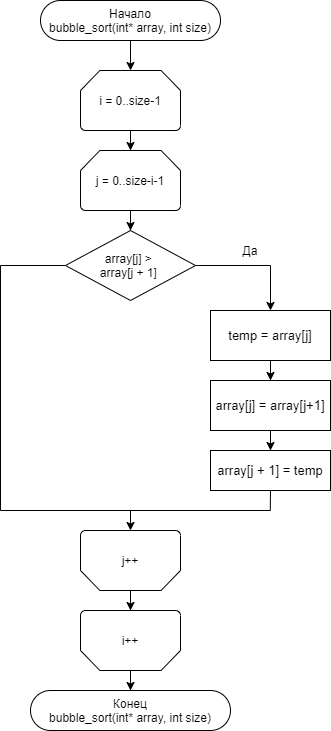
\includegraphics[scale= 0.8]{bubble_sort.png}}
		\caption*{Рисунок 1 - Схема алгоритма сортировки пузырьком}
	\end{figure}
	
	\clearpage
	Ниже на Рисунке 2 изображена схема алгоритма сортировки вставками.
	\begin{figure}[h!]
		\centering{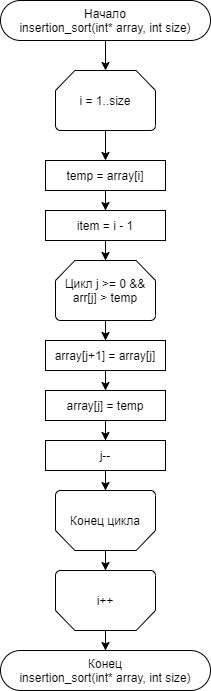
\includegraphics[scale= 0.8]{ins.png}}
		\caption*{Рисунок 2 - Схема алгоритма сортировки вставками}
	\end{figure}

	\clearpage
	Ниже на Рисунке 3 показана схема алгоритма сортировки выбором.
	\begin{figure}[h!]
		\centering{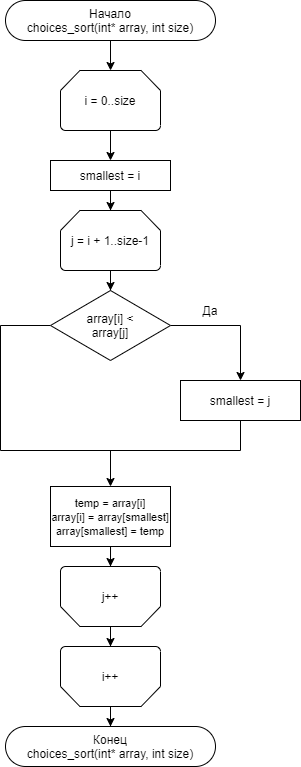
\includegraphics[scale= 0.8]{choices.png}}
		\caption*{Рисунок 3 - Схема алгоритма сортировки выбором}
	\end{figure}
	
	\clearpage
	\subsection{Трудоемкость алгоритмов}
	Введем модель трудоемкости для оценки алгоритмов: 
	\begin{itemize}
		\item[1)] Операции, чья стоимость 1: $=, +, *, \simeq, <, >, \geq, \leq, ==, !=, [], +=, -=, *=, /=, ++, --$;
		\item[2)] стоимость цикла:\par
		$f_{for}=f_{init}+f_{comp}+M(f_{body}+f_{increment}+f_{comp})$\par
		Пример: $for(i=0,i<M;i++){/* body */}$\par
		Результат: $2 + M(2+f_{body})$;
		\item[3)] стоимость условного оператора\par
		Пусть goto (переход к одной из ветвей) стоит 0, тогда\par
		\begin{displaymath}
			f_{f} = \left\{ \begin{array}{l l}
				min(f_{A},f_{B}), & \textrm{лучший случай}\\
				max(f_{A},f_{B}), & \textrm{худший случай}\\
			\end{array} \right.
		\end{displaymath}
	\end{itemize}
	\par Оценим трудоемкость алгоритмов.
	
	\subsubsection{Трудоемкость общей первичной проверки}
		Трудоемкость проверки $if (size <= 0) { return; }$   - 1.
		
	\subsubsection{Трудоемкость алгоритма сортировки пузырьком}
	Внутренний цикл будет выполняться: $n-0-1,n-1-1,n-2-1,...,n-(n-2)-1$ раз. Эта последовательность является арифметической прогрессией и ее можно записать как:\par
	\begin{displaymath}
		s_{bubble}=\frac{(n-1)n}{2}
	\end{displaymath}\par

	Расчет лучшего случая (массив отсортирован): 
	
	
	
	
	
	\clearpage
	\section{Технологическая часть}
	В данном разделе даны общие требования к программе, средства реализации и реализация алгоритмов. 
	
	\subsection{Общие требования к программе}
	Требования к вводу:
	\begin{enumerate}
		\item[1)] возможность ввода размера массива;
		\item[2)] ввод или автоматическая генерация массива. 
	\end{enumerate}
	Требования к программе:
	\begin{enumerate}
		\item[1)] при вводе неправильных размеров массива программа не должна завершаться аварийно;
		\item[2)] корректная сортировка массива. 
	\end{enumerate}

	\subsection{Средства реализации}
	В лабораторной работе был использован язык $C$++\hyperref[CPlusPlus]{[1]}, так как он известен, и на нём было написано множество предыдущих работ.
	
	Среда разработки - $Qt$\hyperref[Cute]{[2]}.
	
	Для замеров процессорного времени была использована функция $clock()$\hyperref[CLOCK]{[3]}.
	\newpage
	
	
	
	\subsection{Реализация алгоритмов}
	В Листинге 1 показана реализация алгоритма сортировки пузырьком.
	
	Листинг 1 -	Алгоритма сортировки пузырьком
	\begin{lstlisting}
		void bubble_sort(int* array, int size)
		{
			if (size <= 0)
			{
				std::cout << "Incorrect array" << std::endl;
				return;
			}
			
			for (int i = 0; i < size - 1; i++)
			{
				for (int j = 0; j < size - i - 1; j++)
				{
					if (array[j] > array[j + 1])
					{
						int temp = array[j];
						array[j] = array[j + 1];
						array[j + 1] = temp;
					}
				}
			}
		}
	\end{lstlisting}
	\newpage
	
	В Листинге 2 описана реализация алгоритма сортировки вставками.
	
	Листинг 2 - Алгоритм сортировки вставками
	\begin{lstlisting}	
		void insertion_sort(int *array, int size)
		{
			if (size <= 0)
			{
				std::cout << "Incorrect array" << std::endl;
				return;
			}
			
			for (int i = 1; i < size; i++)
			{
				int temp = array[i];
				int item = i - 1;
				while(item >= 0 && array[item] > temp)
				{
					array[item + 1] = array[item];
					array[item] = temp;
					item--;
				}
			}
		}	
	\end{lstlisting}
	\newpage
	
	В Листинге 3 описана реализация алгоритма сортировки выбором.
	
	Листинг 3 - Алгоритм сортировки выбором
	\begin{lstlisting}
		void choices_sort(int* array, int size)
		{
			if (size <= 0)
			{
				std::cout << "Incorrect array" << std::endl;
				return;
			}
			
			for (int i = 0; i < size - 1; i++)
			{
				int smallest = i;
				for (int j = i + 1; j < size; j++)
				{
					if (array[j] < array[smallest])
					smallest = j;
				}
				int temp = array[i];
				array[i] = array[smallest];
				array[smallest] = temp;
			}
		}		
	\end{lstlisting}
	\newpage
	
	\subsection*{Вывод}
	\addcontentsline{toc}{subsection}{Вывод}
	По итогу, написанная программа соотвествует всем описанным выше требованиям, алгоритмы были реализованы на C++, так как данный язык известен, выполнено на нём много прошлых работ. 
	
	\clearpage
	\section{Экспериментальный раздел}
	В данном разделе представлены результаты работы программы и приведен анализ времени работы кажого из алгоритмов.
	
	\subsection{Примеры работы программы}
	На Рисунке 4 представлены меню и ввод массива.
	\begin{figure}[h]
		\centering{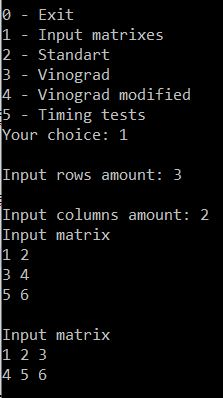
\includegraphics{input.jpg}}
		\caption*{Рисунок 4 - Меню выбора и ввод массива}
	\end{figure}
	
	\newpage
	На Рисунке 5 можно увидеть пример работы всех алгоритмов
	\begin{figure}[h]
		\centering{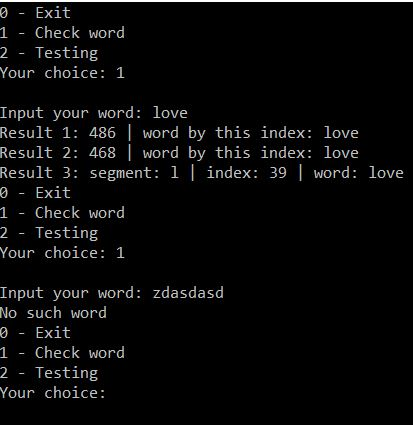
\includegraphics{example.jpg}}
		\caption*{Рисунок 5 - Пример работы всех алгоритмов}
	\end{figure}


	\subsection{Анализ времени работы алгоритмов }
	Эксперементы проводятся на массивах длин 100, 200, 300, 400, 500 элементов. Элементы массива заполняются произвольно.
	
	В первом случае берутся заранее отсортированные массивы. 
	Графики зависимости времени работы алгоритмов от размеров массивов изображены на Рисунке 6.
	
	%\newpage
	\begin{tikzpicture}
		
		\begin{axis}[
			axis lines = left,
			xlabel = Размер массива,
			ylabel = {Кол-во тиков},
			legend pos=north east,
			ymajorgrids=true,
			xmajorgrids=true,
			width = 400
			]
			\addplot[color=red, mark=*] table[x index=0, y index=1] {Bubble1.dat}; 
			\addplot[color=blue, mark=*] table[x index=0, y index=1] {Insertion1.dat};
			\addplot[color=green, mark=*] table[x index=0, y index=1] {Choices1.dat};
			
			\addlegendentry{Bubble}
			\addlegendentry{Insertion}
			\addlegendentry{Choices}
			
		\end{axis}
	\end{tikzpicture}
	\par
	Рисунок 6 -  Графики зависимости времени работы алгоритмов от размеров при заранее отсортированных массивах
	
	\newpage
	Во втором случае берутся обратно отсортированные массивы.
	Графики зависимости времени работы алгоритмов от размеров массивов изображены на Рисунке 7. \par
	
	%\newpage
		\begin{tikzpicture}
			
			\begin{axis}[
				axis lines = left,
				xlabel = Размер массива,
				ylabel = {Кол-во тиков},
				legend pos=north east,
				ymajorgrids=true,
				xmajorgrids=true,
				width = 400
				]
				\addplot[color=red, mark=*] table[x index=0, y index=1] {Bubble2.dat}; 
				\addplot[color=blue, mark=*] table[x index=0, y index=1] {Insertion2.dat};
				\addplot[color=green, mark=*] table[x index=0, y index=1] {Choices2.dat};
				
				\addlegendentry{Bubble}
				\addlegendentry{Insertion}
				\addlegendentry{Choices}
				
			\end{axis}
		\end{tikzpicture}
	\par
	 Рисунок 7 -  Графики зависимости времени работы алгоритмов от размеров при заранее обратно отсортированных массивах
	 
	 \newpage
	 В третьем случае берутся произвольные массивы.
	 Графики зависимости времени работы алгоритмов от размеров массивов изображены на Рисунке 8. \par
	 
	 %\newpage
	 \begin{tikzpicture}
	 	
	 	\begin{axis}[
	 		axis lines = left,
	 		xlabel = Размер массива,
	 		ylabel = {Кол-во тиков},
	 		legend pos=north east,
	 		ymajorgrids=true,
	 		xmajorgrids=true,
	 		width = 400
	 		]
	 		\addplot[color=red, mark=*] table[x index=0, y index=1] {Bubble3.dat}; 
	 		\addplot[color=blue, mark=*] table[x index=0, y index=1] {Insertion3.dat};
	 		\addplot[color=green, mark=*] table[x index=0, y index=1] {Choices3.dat};
	 		
	 		\addlegendentry{Bubble}
	 		\addlegendentry{Insertion}
	 		\addlegendentry{Choices}
	 		
	 	\end{axis}
	 \end{tikzpicture}
	 \par
	 Рисунок 8 -  Графики зависимости времени работы алгоритмов от размеров при произвольно заданных массивах
	 
	 \subsection*{Вывод}
	 \addcontentsline{toc}{subsection}{Вывод}
	 По итогу, все алгоритмы дают верный результат. По значениям замеров можно сделать вывод, что алгоритм сортировки вставками работает быстрее других алгоритмов в большинстве случаях. При обратно отсортированных массивах алгоритм сортировки вставками работает медленнее сортировки выбором. Алгоритм сортировки пузырьком оказался медленнее всех.  
	
	
	\clearpage
	\subsection*{Заключение}
	\addcontentsline{toc}{section}{Заключение}
	В ходе выполнения лабораторной работы были изучены алгоритмы сортировки массивов: пузырьком, вставками и выбором. Были даны теоритические оценки алгоритмов сортировки массиов. Была дана оценека трудоемкости алгоритмов. Также было произведено сравнение времени работы алгоритмов, в результате которого стало очевидно, что алгоритм сортировки вставками примерно в 2 раза быстрее сортировки пузырьком и в 1.2 раза - сортировки выбором (за исключением ситуации обратно отсортированного массива).
	
	\newpage	
	\section*{Литература}
	\addcontentsline{toc}{chapter}{Литература}
		
	\begin{enumerate}
		\label{CPlusPlus}
		\item[1)] Бьерн Страуструп. Язык программирования С++. -URL:\par 
		\href{https://codernet.ru/books/c_plus/bern_straustrup_yazyk_programmirovaniya_c_specialnoe_izdanie/}
		{https://codernet.ru/books/c\_plus/bern\_straustrup\_yazyk\_programmirovaniya\_
			c\_specialnoe\_izdanie/}\par(дата обращения:
		01.10.2020). Текст: электронный.
		
		\label{Cute}
		\item[2)] Qt. -URL:\par
		\href{https://www.qt.io/}{https://www.qt.io/} (дата обращения: 01.10.2020). Текст: электронный.
		
		\label{CLOCK}
		\item[3)] Функция $clock$. -URL:\par
		\href{https://docs.microsoft.com/ru-ru/cpp/c-runtime-library/reference/clock?view=vs-2019}{https://docs.microsoft.com/ru-ru/cpp/c-runtime-library/reference/clock?view=vs-2019} (дата обращения:
		01.10.2020). Текст: электронный.
		
		\label{MatrixInfo}
		\item[4)] Дж. Макконнелл. Основы современных алгоритмов.\newline 2-е дополненное издание
		\newline Москва: Техносфера, 2004. - 368с. ISBN 5-94836-005-9\newline
		с. 130 - 133
		
	\end{enumerate}
\end{document}